\documentclass{beamer}
\usetheme{metropolis}
\usepackage{ctex}

\title{Item-Based Collaborative Filtering}
\date{\today}
\author{Yang LI}
\institute{School of Software Engineering, Tongji University}

\begin{document}
  \maketitle
  \section{Improvement}
  \begin{frame}{Achievement}
    \begin{itemize}
      \item 更新了数据集, 使用了三个月的训练数据
      \begin{itemize}
        \item 相较于上次实验结果, 本次测试结果出现下降
      \end{itemize}
      \item 变化了测试时用户购买商品的种数的阈值
      \item 对于训练集未出现的商品, 在测试集中予以删除
      \begin{itemize}
        \item 可预料的, 提高了recall, 而precision不变
      \end{itemize}
      \item 根据用户测试集中购买的商品种数, 进行推荐(上限为$20$)
      \begin{itemize}
        \item 可预料的, 提高了precision, 而recall不变
      \end{itemize}
    \end{itemize}
  \end{frame}
  
  \begin{frame}{Result}
    \centering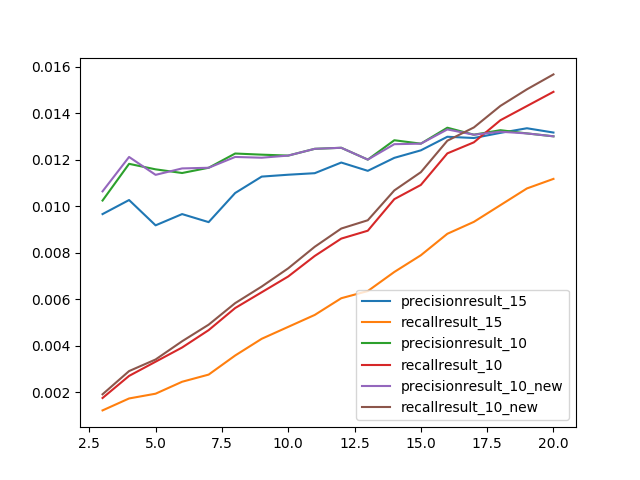
\includegraphics[width=\textwidth]{../result.png}
  \end{frame}
  
  \begin{frame}{Dive into pieces}
    Take User $$
  \end{frame}

\end{document}
